\subsubsection{QuizziPedia::Back-End::App::Routers}

\label{QuizziPedia::Back-End::App::Routers}
\begin{figure}[ht]
	\centering
	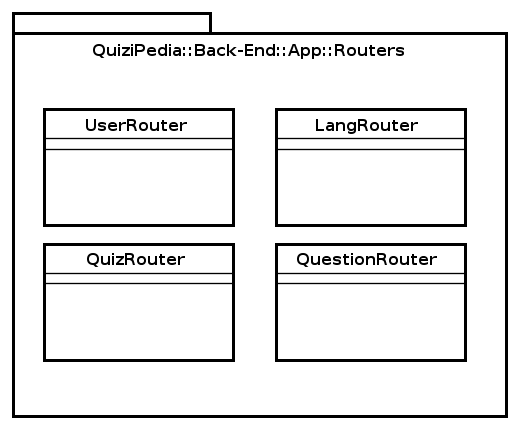
\includegraphics[scale=0.65]{UML/Package/QuizziPedia_Back-End_App_Routers.png}
	\caption{QuizziPedia::Back-End::App::Routers}
\end{figure}
\FloatBarrier
	\begin{itemize}
		\item \textbf{Descrizione}: 
		\textit{package\ped{G}} contenente i router della componente back-end dell'applicazione. Contiene i file di configurazione relativi al routing delle richieste del \textit{client\ped{G}}, ossia i \textit{routers} di \textit{Express\ped{G}};
		\item \textbf{Padre}: \texttt{App};
		\item \textbf{Interazioni con altri componenti}:
			\begin{itemize}
				\item \texttt{Controllers}: \textit{package\ped{G}} che contiene i \textit{Controllers} di \textit{Express\ped{G}}, definisce la logica dell'applicazione.
			\end{itemize}
		\item \textbf{Classi Contenute}:
		\begin{itemize}
			\item \texttt{UserRouter}: classe che gestisce le richieste relative alla registrazione, alla gestione della sessione e alla cronologia dei questionari svolti di un utente. Componente ConcreteHandler del design pattern \textit{Chain of responsibility\ped{G}}. Utilizza il modulo \textit{Passport\ped{G}};
			\item \texttt{QuestionRouter}: classe che gestisce le richieste relative alle operazioni riguardanti le domande. Componente ConcreteHandler del design pattern \textit{Chain of responsibility\ped{G}}. Utilizza il modulo \textit{Passport\ped{G}};
			\item \texttt{QuizRouter}: classe che gestisce le richieste relative alle operazioni riguardanti un questionario;
			\item \texttt{LangRouter}: classe che gestisce le richieste relative alla lingua;
		\end{itemize}
	\end{itemize}
